\documentclass{article}

\usepackage{ai4science_ysda2026}

\usepackage{amsmath}
\usepackage{amssymb}
\usepackage{graphicx}
\usepackage{booktabs}
\usepackage{microtype}

\icmltitlerunning{Корональные дыры и ионосфера}

\begin{document}

\twocolumn[
  \icmltitle{Связь площади областей, подозреваемых на наличие корональных дыр,
  с полным электронным содержанием ионосферы Земли}

  \begin{icmlauthorlist}
    \icmlauthor{Борис Салимов}{org1}
  \end{icmlauthorlist}

  \icmlaffiliation{org1}{Институт солнечно-земной физики Сибирского отделения
  Российской академии наук, ул. Лермонтова, 126а, Иркутск, Россия}

  \icmlcorrespondingauthor{Борис Салимов}{salimov@iszf.irk.ru}

  \icmlkeywords{Солнце, корональные дыры, солнечный ветер, ионосфера,
  полное электронное содержание, Сибирский радиогелиограф}

  \vskip 0.3in
]

\printAffiliationsAndNotice{}

\begin{abstract}
Солнечная активность влияет на ионосферу Земли. Помимо электромагнитного
излучения, на ионосферу воздействует солнечный ветер --- поток заряженных
частиц, ускоряемый, в частности, в корональных дырах. В данной работе
исследована взаимосвязь
областей, похожих на корональные дыры, с полным электронным содержанием
ионосферы (ПЭС). Найдена слабая отрицательная корреляция (коэффициент
корреляции Пирсона) между площадью тёмных областей и параметром ПЭС для
скорости солнечного ветра 800~км/с. Это может говорить как о незначительном
влиянии площади корональных дыр на ионосферу, так и о недостаточно точном
способе определения реальной площади корональных дыр Солнца.
\end{abstract}

\section{Введение}

Солнечная активность влияет на ионосферу Земли. Излучение на длине волны
10.7~см значительно коррелирует с критической частотой ионосферы, от которой
зависят режимы работы средств радиосвязи и навигации \citep{tapping2013f107}.
Однако электромагнитное излучение --- не единственный фактор, воздействующий
на ионосферу Земли.

Существует также солнечный ветер --- непрерывный поток заряженных частиц
(разреженной плазмы), который истекает из внешней атмосферы Солнца (короны)
в межпланетное пространство со скоростью от 300 до 1200~км/с. Из корональных
дыр исходят самые быстрые потоки солнечного ветра \citep{cranmer2019properties}.
В работе изучена корреляция областей, которые подозреваются на наличие
корональных дыр по данным Сибирского радиогелиографа, с важным показателем
ионосферы --- полным электронным содержанием \citep{afraimovich2008gec}.

\section{Данные}

Использовался ряд данных глобального электронного содержания (GEC, далее
обозначается ПЭС), полученный с сайта SIMuRG \citep{simurg2025}; система
SIMuRG описана в работе
\citet{yasyukevich2020simurg}. Ряд охватывает 2025~год; исходные значения
ПЭС имеют 15-минутное разрешение.

На рисунке~\ref{fig:gec} приведён весь использованный ряд ПЭС за 2025~год.
Виден характерный сезонный ход: значения ПЭС повышены в конце зимы и весной,
достигая максимума в апреле, а летом (июнь--июль) опускаются до минимальных
значений около 1~TECU. Осенью ПЭС вновь возрастает, и до конца года
сохраняется повышенный уровень. На этом медленном сезонном фоне заметны
короткие всплески и провалы длительностью от нескольких часов до нескольких
суток, связанные с геомагнитными возмущениями. Разрыв в ряду в конце ноября
соответствует отсутствию данных за 26~ноября 2025~г.

\begin{figure*}[t]
\centering
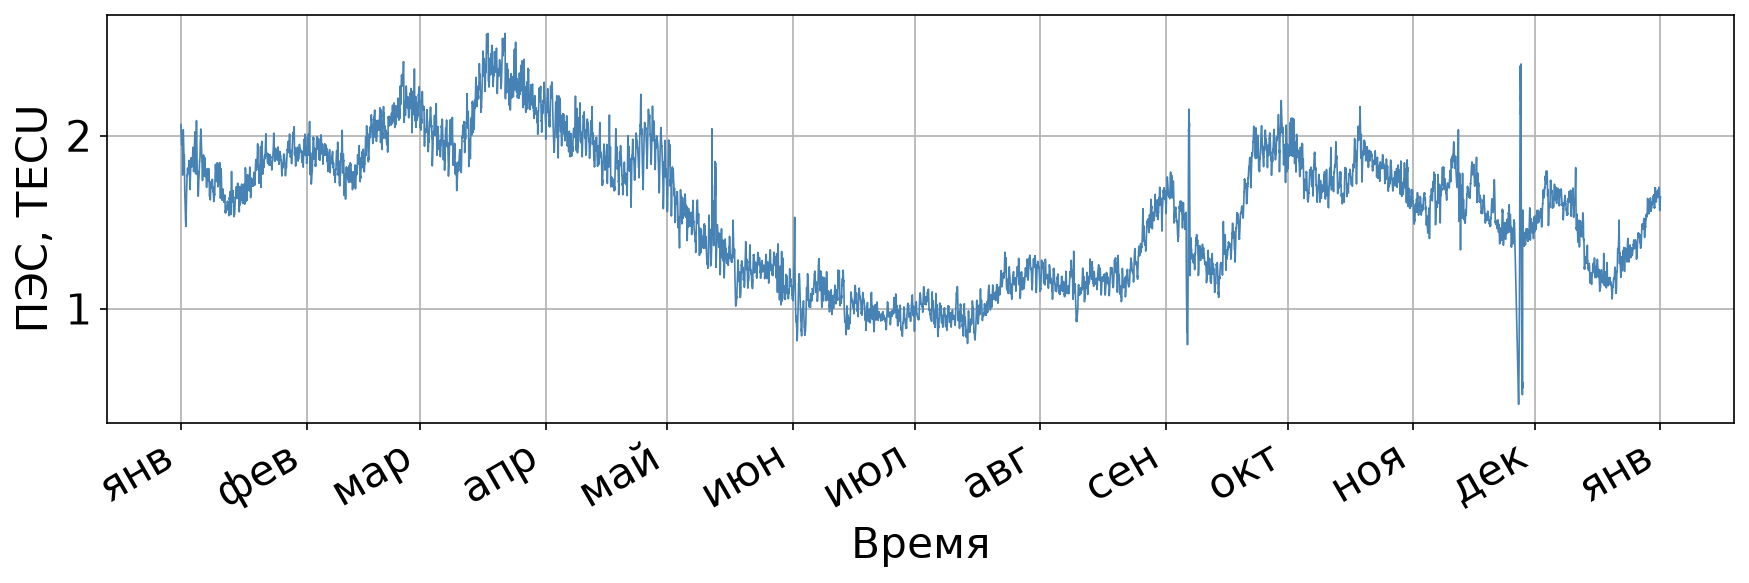
\includegraphics[width=\textwidth]{figures/gec.png}
\caption{Полное электронное содержание (ПЭС) за 2025~год по данным SIMuRG:
15-минутный ряд, значения в TECU.}
\label{fig:gec}
\end{figure*}

Обработанные радиоизображения Солнца в радиодиапазоне 3~ГГц получены по данным
Сибирского радиогелиографа \citep{lesovoi2017srh}. Изображения использовались
усреднёнными за час для моментов 03:00~UT и 07:00~UT. Например, для момента 03:00~UT значения яркостной
температуры высчитывались как среднее значение за период с 02:30~UT по 03:30~UT

Площади, подозреваемые на корональные дыры, отбирались как области со
значениями яркостной температуры меньше определённого порога. Полученная площадь выражается в долях
площади солнечного диска и в используемом ряду является безразмерной
величиной.

Порог высчитывался как яркостная температура спокойного Солнца. Яркостная температура
спокойного Солнца считалась как наиболее вероятная (мода) по гистограмме значений всех пикселей.

\begin{figure}[t]
\centering
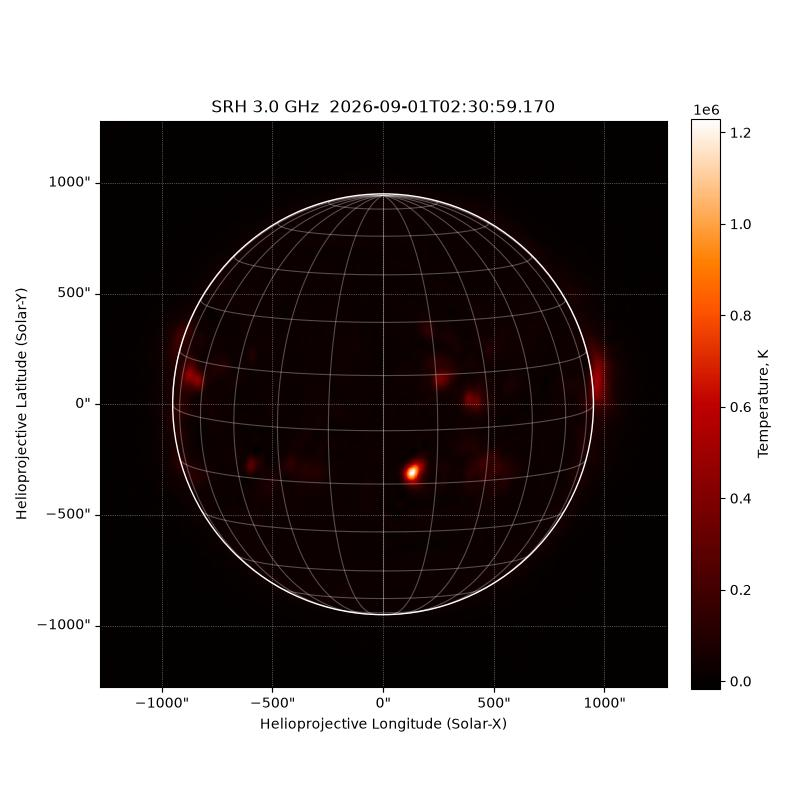
\includegraphics[width=\columnwidth]{figures/solar_without_process.jpg}
\caption{Пример исходного радиоизображения Солнца на частоте 3~ГГц по данным
Сибирского радиогелиографа: показана яркостная температура в кельвинах и
нанесена гелиопроекционная сетка.}
\label{fig:solar-raw}
\end{figure}

На рисунке~\ref{fig:solar-raw} приведён пример исходного радиоизображения
Солнца, по которому строился ряд площадей. Видно, что тёмные области
занимают лишь часть диска, а их выделение требует выбора порога яркостной
температуры.


Всего в ряду площадей содержится 722 момента времени. Для двух из них
(03:00~UT и 07:00~UT 26~ноября 2025~г.) значения ПЭС в использованном ряду
отсутствуют, поэтому непосредственно сопоставить удалось 720 моментов.

\section{Методология}

Так как солнечный ветер достигает поверхности Земли с задержкой, его корреляция
рассчитывалось со сдвинутым рядом ПЭС на время, за которое солнечный ветер
достигнет поверхности Земли. Время переноса для каждого момента $t_i$
оценивалось как
\begin{equation}
\Delta t_i = \frac{R(t_i)}{v},
\label{eq:delay}
\end{equation}
где $R(t_i)$ --- расстояние Солнце--Земля в момент $t_i$, а $v$ --- скорость
солнечного ветра. Расстояние $R(t_i)$ рассчитывалось по приближённой формуле
земной орбиты; его среднее значение за рассматриваемый период составило
1.00037~а.е.

Средняя скорость солнечного ветра принималась равной 800~км/с. Для быстрых
потоков, связанных с корональными дырами, скорость у~1~а.е. достигает
700--900~км/с \citep{cranmer2019properties}, поэтому значение 800~км/с
использовано как характерная оценка. При такой скорости средняя задержка
составляет 2.165~сут.

Значения ПЭС в сдвинутые моменты $t_i+\Delta t_i$ были получены линейной
интерполяцией исходного ряда. Пары, выходящие за пределы ряда или
пересекающие разрыв длиной более 24~ч, были исключены. Для оставшихся пар
рассчитывался коэффициент корреляции Пирсона между площадью областей, подозреваемых на наличие
корональных дыр
$A_i=A(t_i)$ и значением ПЭС $G_i=G(t_i+\Delta t_i)$:
\begin{equation}
\begin{aligned}
r = \frac{\sum_{i=1}^{N}(A_i-\bar{A})(G_i-\bar{G})}
{\sqrt{\sum_{i=1}^{N}(A_i-\bar{A})^2}\,
 \sqrt{\sum_{i=1}^{N}(G_i-\bar{G})^2}},
\end{aligned}
\label{eq:pearson}
\end{equation}
где $N$ --- число пар, $\bar{A}$ и $\bar{G}$ --- средние значения
соответствующих рядов.

\section{Результаты}

После сдвига ряда и исключения пар, для которых интерполяция невозможна,
осталось $N=711$ пар. Коэффициент корреляции Пирсона между площадью
областей, похожих на корональные дыры, и параметром ПЭС для скорости
солнечного ветра 800~км/с оказался равным
\begin{equation}
r = -0.272352.
\label{eq:result}
\end{equation}
Основные параметры расчёта приведены в таблице~\ref{tab:result}.

\begin{table}[t]
\centering
\caption{Параметры корреляционного анализа площади областей, похожих на
корональные дыры, и ПЭС.}
\label{tab:result}
\small
\setlength{\tabcolsep}{4pt}
\begin{tabular}{p{0.62\columnwidth}l}
\toprule
Параметр & Значение \\
\midrule
Скорость солнечного ветра $v$ & 800~км/с \\
Среднее расстояние Солнце--Земля $R$ & 1.00037~а.е. \\
Средняя задержка $\Delta t$ & 2.165~сут \\
Число пар $N$ & 711 \\
Коэффициент корреляции Пирсона $r$ & $-0.272$ \\
Коэффициент детерминации $r^2$ & 0.074 \\
\bottomrule
\end{tabular}
\end{table}

Коэффициент отрицательный и невысок сам по себе: квадрат коэффициента
корреляции составляет примерно 0.074, то есть линейная связь объясняет лишь
около 7\,\% дисперсии. Полученный результат означает, что площадь областей,
похожих на корональные дыры, определённая по имеющимся радиоизображениям,
сама по себе не является сильным определяющим параметром ПЭС.

\section{Обсуждение}

Слабая отрицательная корреляция допускает несколько интерпретаций.
Во-первых, она может указывать на незначительный вклад площади корональных
дыр в изменение ПЭС по сравнению с другими источниками ионосферной
изменчивости. Во-вторых, отрицательный знак может быть следствием
недостаточно точного определения реальной площади корональных дыр: пороговая
сегментация радиоизображений чувствительна к выбору порога и условиям
наблюдений.



Слабая корреляция не означает, однако, что связи между корональными дырами
и ионосферой нет. На 9-дневные колебания нейтральной плотности термосферы Земли в 2005 и 2006
годах повлияли вращающиеся корональные дыры и квазипериодические высокоскоростные
потоки солнечного ветра, а также сопутствующая им периодическая геомагнитная активность \citep{fang2012recurrent}.


Субгармонические колебания электронной плотности ионосферы на дневной и
ночной сторонах хорошо коррелируют с колебаниями скорости солнечного ветра
и индекса $Kp$ в 2008~г.\ \citep{tulasiram2010periodic}.

В отдельных событиях
корональная дыра оказывается источником сильной магнитной бури, а
высокоскоростной поток воздействует на Землю несколько суток
\citep{shimeis2012signature}.

Потоки из корональных дыр создают колебания
модуля межпланетного магнитного поля, приводящие к геомагнитным возмущениям
на высоких широтах и к отклику ионосферы \citep{liu2019analyzing}.

Даже не очень сильное событие, связанное с корональной дырой, может вызывать заметные
изменения ПЭС, электронной концентрации и параметров экваториальной
ионосферы \citep{younas2022ionospheric}.


Перечисленные работы, однако, основаны на событийном анализе или на
выделении квазипериодического отклика в ограниченные интервалы времени.
В настоящей работе анализируется годовой ряд, а значение ПЭС явяется характеристикой
всей ионосферы.

В качестве ограничений работы можно отметить, что при глобальном усреднении,
часть эффектов может взаимно
компенсироваться. Тогда как в работах \citep{liu2019analyzing,tulasiram2010periodic} отклик ионосферы на высокоскоростные потоки локализован
по широте и местному времени.


Кроме того, в расчёте использовалась единая скорость
солнечного ветра 800~км/с, тогда как реальная скорость меняется от события
к событию. Само ПЭС зависит не только от корональных дыр, но и от других
факторов солнечной и геомагнитной активности. Наконец, временное разрешение
ряда площадей составляет всего два отсчёта в сутки, что ограничивает
возможность точного учёта задержки.

Площадь и позиция корональной дыры является важным параметром. По данным спутников
ACE и STEREO пиковые скорости высокоскоростных потоков сильно зависят как
от площади, так и от ко-широты их солнечного источника относительно
гелиосферной широты измеряющего спутника, поэтому ко-широта корональной
дыры важна для предсказания свойств потока вблизи Земли
\citep{hofmeister2018dependence}. Площадь корональной дыры
следует учитывать, но одной площади недостаточно.
В использованном ряду площадь областей, похожих на корональные дыры,
не сопровождается сведениями об их положении на диске Солнца, поэтому один
и тот же прирост площади может соответствовать разным условиям прихода
потока к Земле. Это дополнительно ослабляет ожидаемую корреляцию площади
с ПЭС и затрудняет интерпретацию её знака.

Для повышения точности определения площади корональных дыр
по данным Сибирского радиогелиографа и для корректного сопоставления с ПЭС
необходимы дальнейшие исследования и разработка моделей машинного обучения,
способных устойчиво выделять корональные дыры на радиоизображениях, а также
учёт положения корональных дыр на диске Солнца и оценок скорости солнечного
ветра для каждого события.

\section{Заключение}

В работе исследована связь площади областей, похожих на корональные дыры,
с полным электронным содержанием ионосферы. Для скорости солнечного ветра
800~км/с получен коэффициент корреляции Пирсона $r=-0.272$ при $N=711$.
Корреляция слабая и отрицательная. Это может говорить как о незначительном
влиянии площади корональных дыр на ионосферу, так и о недостаточно точном
способе определения реальной площади корональных дыр Солнца. Для уточнения
результата необходимы более точная сегментация корональных дыр и дальнейшее
развитие моделей машинного обучения. Исходный код исследования находится
по ссылке \anonymized{\url{https://github.com/BorisSalimov87/solar_influence/tree/build_article}}.

\begin{aiusage}[Укажите фрагменты, порождённые моделью или взятые из
  источников, и способ их проверки.]
  Обсуждение & \porozhdeno{} & deepseek/ deepseek-v4.1-flash-1017
    & утверждения сверены с работами, скорректировано \\
  Остальной текст & \napisano{} & --- & --- \\
\end{aiusage}

\bibliographystyle{ai4science_ysda2026}
\bibliography{references}

\end{document}
